\documentclass[11pt,letterpaper]{article}

\usepackage[margin=1in]{geometry}
\usepackage{amsmath,amssymb}
\usepackage{graphicx}
\usepackage{booktabs}
\usepackage{hyperref}
\usepackage{float}
\usepackage{caption}

\title{\textbf{HWRS640 -- Assignment 3:\\Convolutional Neural Networks for Satellite Image Segmentation}}
\author{Nabin Kalauni}
\date{April 6, 2026}

\begin{document}
\maketitle

% ===========================================================================
\section{Problem 1: Data Exploration and Preprocessing (20 pts)}
% ===========================================================================

\subsection{Dataset Structure}

The \texttt{nikolkoo/SatelliteSegmentation} dataset contains 790 RGB satellite images of size $256\times256$, each paired with a pixel-wise segmentation mask of the same size. Mask values are ESA WorldCover class codes: 0, 10, 20, 30, 40, 50, 60, 70, 80, 90, 100 -- giving \textbf{11 classes} in total. These were remapped to contiguous indices $0,\ldots,10$ before training.

\subsection{Sample Visualisations}

Figure~\ref{fig:samples} shows five image--mask--overlay triplets drawn from the training split, using a consistent \texttt{tab20} colormap so the same class always appears in the same colour.

\begin{figure}[H]
    \centering
    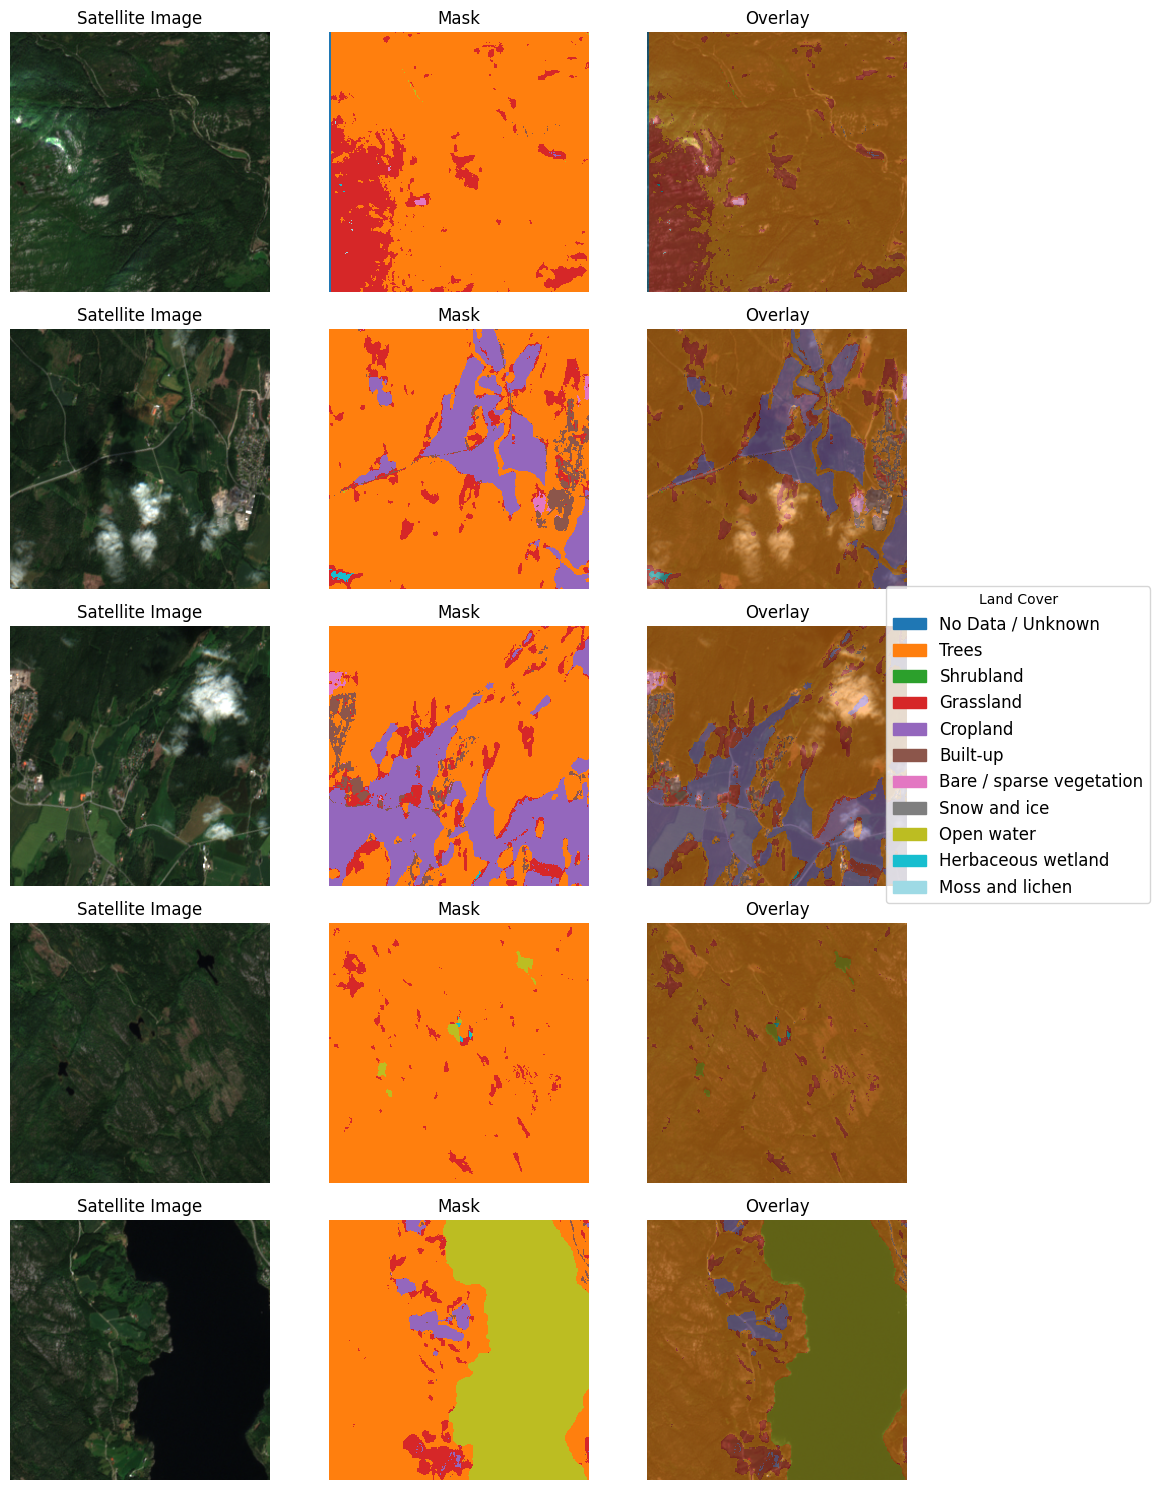
\includegraphics[width=0.85\textwidth]{satellite_samples.png}
    \caption{Five sample image--mask--overlay triplets from the training set.}
    \label{fig:samples}
\end{figure}

\subsection{Class Balance}

\begin{figure}[H]
    \centering
    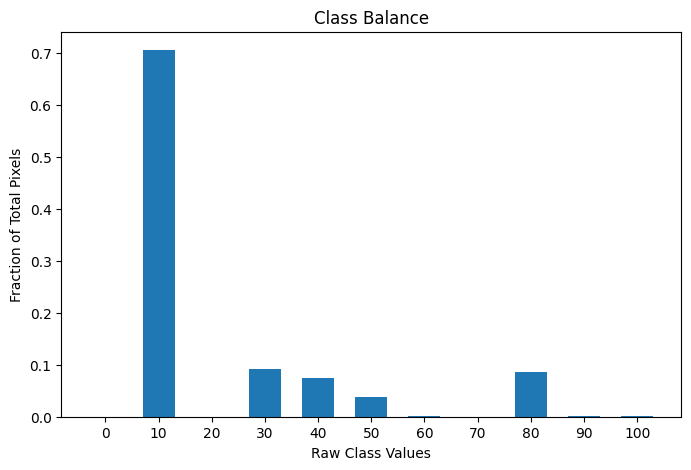
\includegraphics[width=0.75\textwidth]{class_balance.png}
    \caption{Fraction of all pixels belonging to each ESA WorldCover class.}
    \label{fig:balance}
\end{figure}

The class distribution is highly skewed (Figure~\ref{fig:balance}): Trees (class 10) accounts for $\sim$70.6\% of all pixels, while several classes such as Shrubland (20, $\sim$0.003\%) and Snow/Ice (70, $<$0.0001\%) are nearly absent. A naive classifier that predicts ``Trees'' everywhere would achieve high pixel accuracy while completely failing on rare classes. This motivates the use of inverse-frequency class weights in the loss function to prevent the model from ignoring minority classes during training.

\subsection{Dataset and DataLoader}

The dataset was split 80/20 into training (632 samples) and validation (158 samples) sets. Each image was normalised to a $[0,1]$ \texttt{float32} tensor of shape $(3,256,256)$; masks were resized with nearest-neighbour interpolation and cast to \texttt{int64} with values in $\{0,\ldots,10\}$.

% ===========================================================================
\section{Problem 2: Model Design and Implementation (25 pts)}
% ===========================================================================

\subsection{Architecture}

A U-Net encoder--decoder with skip connections was implemented. The encoder has four downsampling stages with feature widths $[32, 64, 128, 256]$, each consisting of two $3\times3$ convolutions followed by BatchNorm and ReLU (a ``DoubleConv'' block), then $2\times2$ max-pooling. The bottleneck applies another DoubleConv at 512 channels. The decoder mirrors the encoder, using transposed convolutions for $2\times$ upsampling and concatenating the corresponding encoder skip features before each DoubleConv block. A final $1\times1$ convolution maps 32 channels to 11 class logits.

\subsection{Architectural Justification}

A standard classification CNN progressively discards spatial information through pooling, culminating in a global feature vector -- unsuitable for pixel-wise prediction. U-Net preserves full-resolution spatial context by passing encoder feature maps directly to the decoder via skip connections. These connections allow the decoder to combine coarse semantic features from the bottleneck with fine-grained spatial detail from early encoder layers, which is critical for accurate boundary delineation in segmentation. The encoder--decoder design also ensures the output has the same spatial extent as the input without any fully connected layers.

\subsection{Parameter Count}

\[
    \text{Total trainable parameters} = \mathbf{7{,}763{,}371}
\]

% ===========================================================================
\section{Problem 3: Training (25 pts)}
% ===========================================================================

The model was trained for 80 epochs using AdamW with an initial learning rate of $10^{-3}$ and a \texttt{ReduceLROnPlateau} scheduler (patience 5). Pixel-wise cross-entropy loss was used with inverse-frequency class weights:
\[
    w_c = \frac{\text{total pixels}}{C \times \text{pixels of class } c}
\]
The best model checkpoint (by validation mIoU) was saved and used for all subsequent evaluation.

\begin{figure}[H]
    \centering
    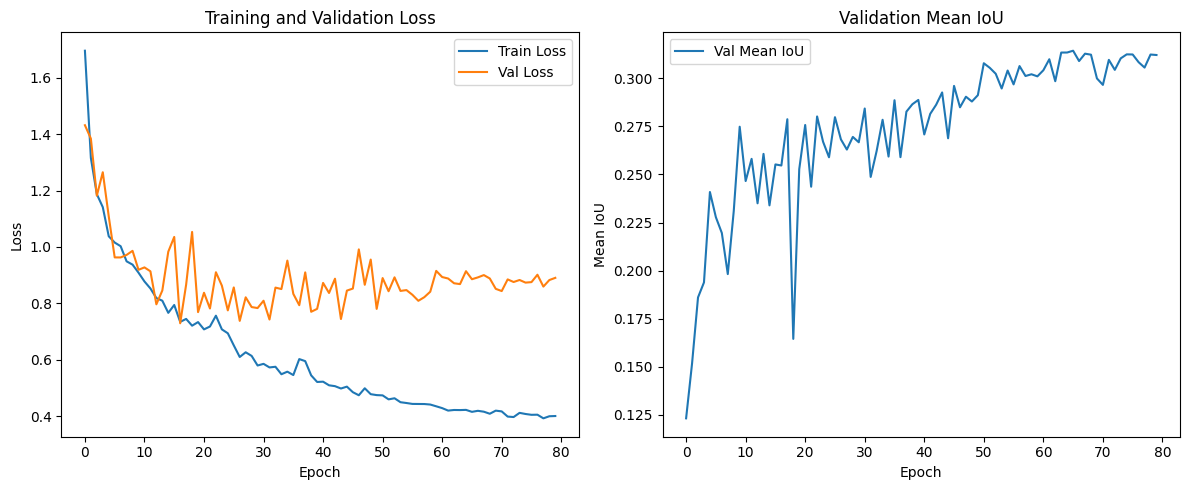
\includegraphics[width=\textwidth]{training_curves.png}
    \caption{Left: training and validation loss vs.\ epoch. Right: validation mean IoU vs.\ epoch.}
    \label{fig:curves}
\end{figure}

The model shows mild overfitting: training loss decreases steadily from $\sim$1.73 to $\sim$0.39 by epoch 80, whereas validation loss plateaus around 0.85--0.90 after epoch 50 while continuing to fluctuate. Nevertheless, validation mIoU improves throughout, reaching a best of \textbf{0.4079} at epoch 72, suggesting the model is still learning useful representations rather than simply memorising the training set.

% ===========================================================================
\section{Problem 4: Evaluation and Interpretation (30 pts)}
% ===========================================================================

\subsection{4a. Quantitative Evaluation}

The best saved model was evaluated on the full validation set:

\[
    \text{mIoU} = \mathbf{0.3212}
\]

\begin{figure}[H]
    \centering
    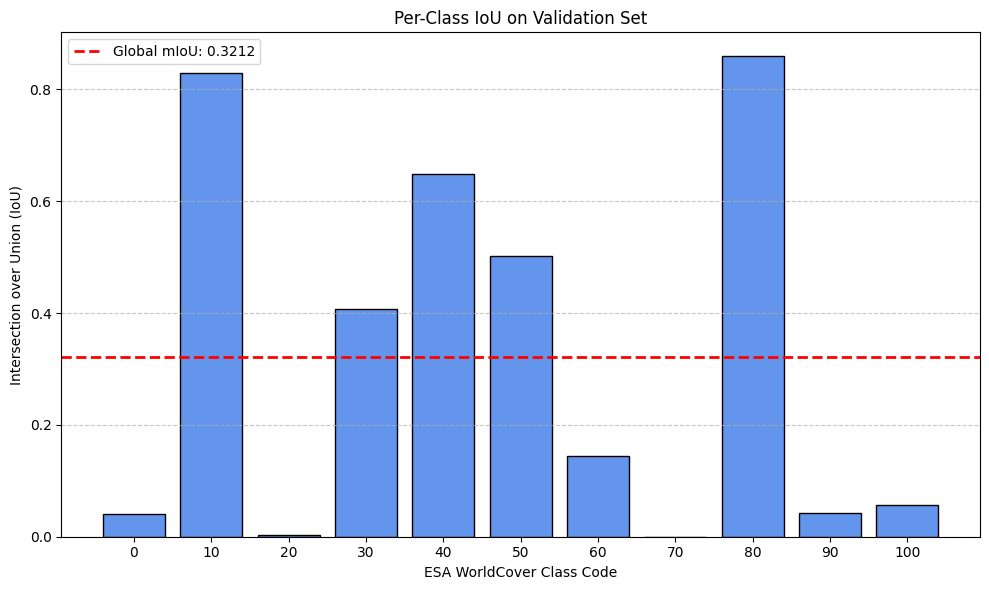
\includegraphics[width=0.85\textwidth]{iou_per_class.png}
    \caption{Per-class IoU bar chart (produced inline in the notebook). The dashed red line marks the global mIoU of 0.3212.}
    \label{fig:iou_bar}
\end{figure}

The model performs well on the four dominant classes -- Trees (10), Grassland (30), Cropland (40), and Open Water (80) -- which together comprise $\sim$97\% of pixels. Rare classes such as Shrubland (20), Snow/Ice (70), Herbaceous Wetland (90), and Moss/Lichen (100) achieve near-zero IoU. This directly mirrors the class imbalance found in Problem 1: even with inverse-frequency weighting, the model sees too few examples of extreme minority classes to learn reliable boundaries for them, and their near-zero IoU pulls the mIoU down considerably.

\subsection{4b. Qualitative Evaluation}

\begin{figure}[H]
    \centering
    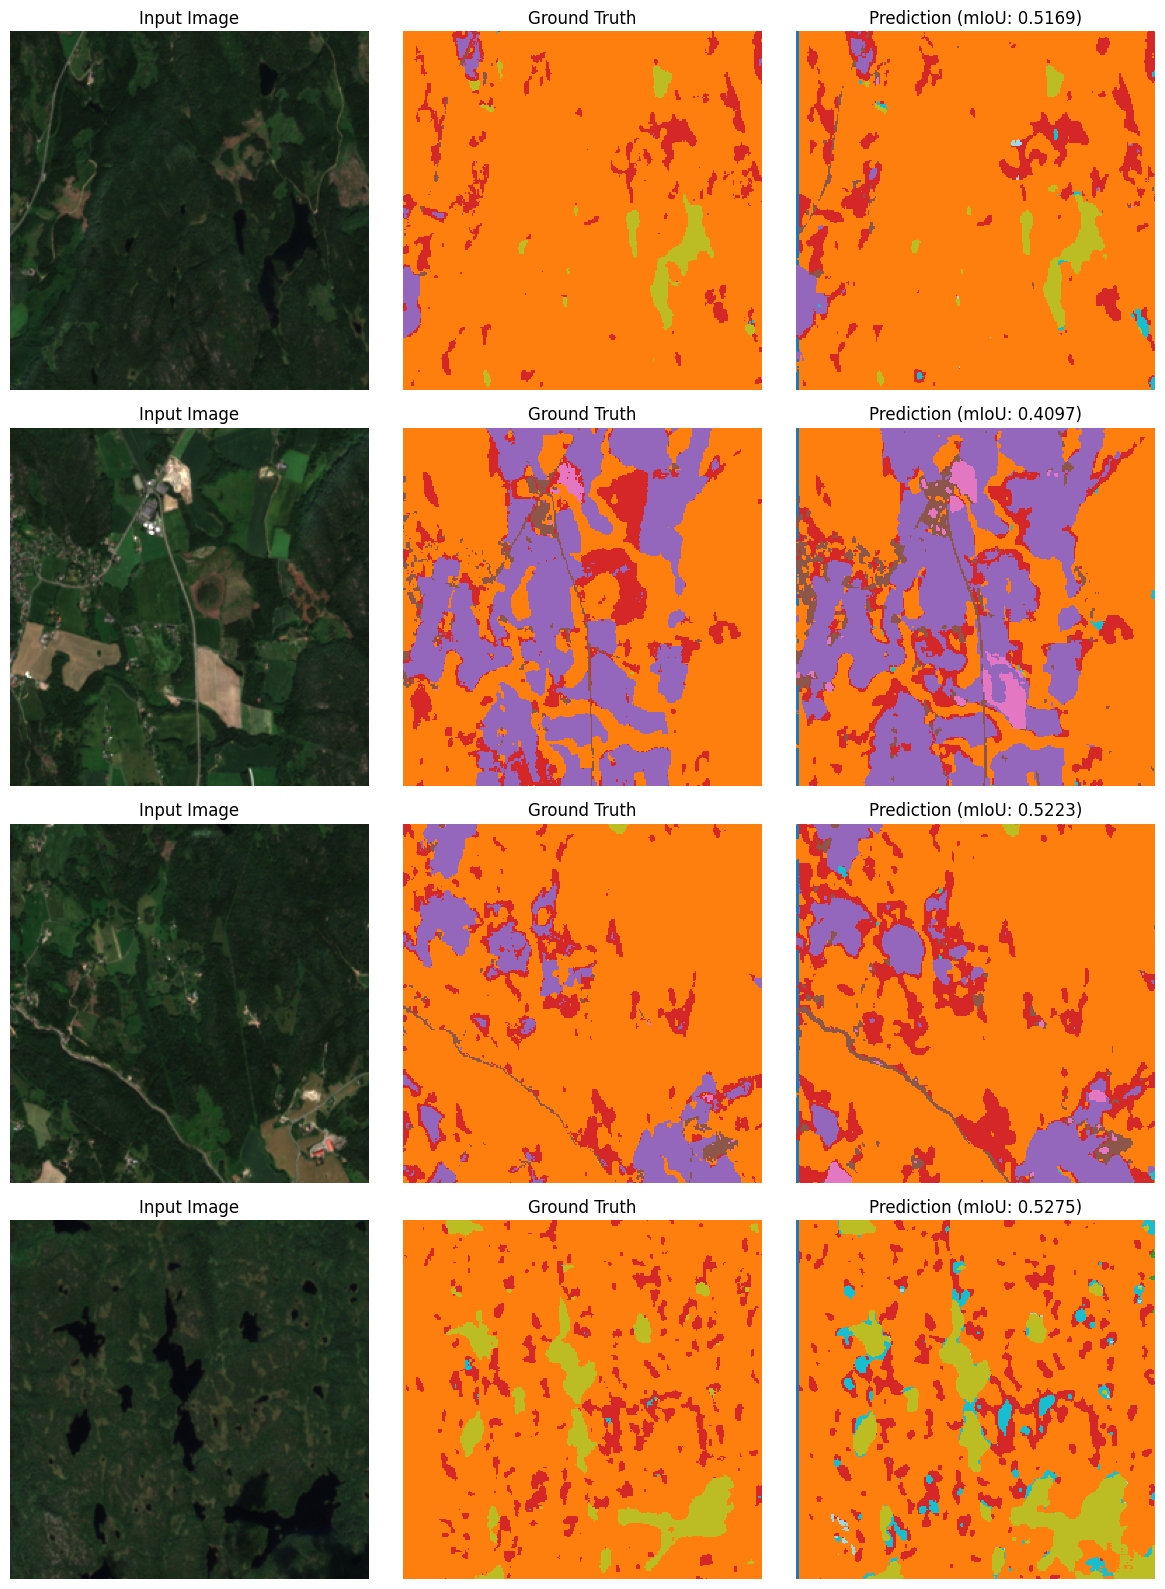
\includegraphics[width=\textwidth]{sample_predictions.png}
    \caption{Four validation samples: input image (left), ground-truth mask (centre), predicted mask (right). Per-sample mIoU is shown in each prediction title.}
    \label{fig:preds}
\end{figure}

\textbf{Success case.} Samples with large, homogeneous regions of Trees or Open Water are predicted with high mIoU ($>0.5$). The model correctly segments broad spectral signatures -- dark blue water, dense green canopy -- where the class boundary is spectrally sharp.

\textbf{Failure case.} Samples containing rare classes (Shrubland, Wetland) or fine-grained urban patterns (Built-up, class 50) are systematically mislabelled, often as Trees or Grassland. These classes share similar spectral reflectance profiles and lack sufficient training examples for the model to learn discriminative features, leading to low per-sample mIoU.

\subsection{4c. Reflection}

\textbf{IoU vs.\ pixel accuracy.} Pixel accuracy rewards the classifier for correctly labelling abundant classes and tolerates complete failure on rare ones. In this dataset, a model predicting only Trees achieves $\sim$70.6\% pixel accuracy while IoU for every other class is zero. IoU forces the metric to be non-zero only when the model correctly identifies the spatial extent of each class, so each class contributes equally to the mean regardless of how few pixels it occupies. This makes mIoU a far more informative measure of segmentation quality when classes are imbalanced.

\textbf{Pretrained encoder.} Using a ResNet backbone pretrained on ImageNet would very likely improve performance, especially on rare classes. Pretrained features capture low-level textures (edges, colour gradients) and mid-level patterns (object parts, textures) that generalise across domains. Although satellite imagery differs from natural photos in viewing angle and spectral content, the convolutional filters for detecting vegetation texture, water reflectance, and built structure boundaries are meaningfully shared. The pretrained encoder also initialises the network in a good region of weight space, enabling faster convergence and better generalisation from the limited 790-sample dataset.

\end{document}
